\documentclass[xcolor=dvipsnames,10pt]{beamer}
% ********** Styl prezentacji **********
\mode<presentation>
{
	\usetheme{Warsaw}
}

\author{Mahmoud Fatene \\ Frederic Durand \\ Valene Pellissier \\ Claire Yang}
%\institute[...]{...}

%\addtobeamertemplate{footline}{\insertframenumber}
\subject{}
\AtBeginSubsection[]
{
	\begin{frame}<beamer>
		\frametitle{Table of Contents}
		\tableofcontents[currentsection,currentsubsection]
	\end{frame}
}

\title[Master Project]{Master Project}
\subtitle{Water Sterilizer Optimization}

\date{January 2008}

%\AtBeginSubsection[]{
%	\begin{frame}<beamer>
%		\frametitle{Outline}
%		\addtocounter{framenumber}{-1}
%		\thispagestyle{empty}
%		\tableofcontents[currentsection]
%	\end{frame}
%}
\begin{document}


\begin{frame}
	\titlepage
	\begin{figure}
	\raggedleft
	
\includegraphics[height=1cm, width=2cm]{./images/logoUJF.jpg}
	\hspace{65mm}
	\raggedright
	
\includegraphics[height=1.3cm, width=2cm]{./images/logoRCLux.jpg}
	\end{figure}
\end{frame}

\begin{frame}
	\frametitle{Table of contents}
	\tableofcontents
\end{frame}

%%%%%%%%%%%%%%%%%%%%%%%%%Subject%%%%%%%%%%%%%%%%%%%%%%%%%%%%%%%%%%

\section{Subject}

\begin{frame}
	\frametitle{Definition}
\begin{itemize}[<+->]
\item \textbf{Context:} To model water sterilization by UV radiation with this device :
	\begin{figure}
		\raggedleft
		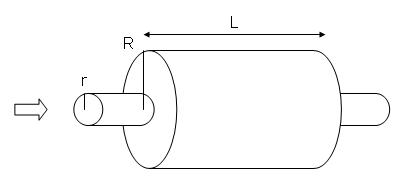
\includegraphics[width=5cm,height=2cm]{./images/sterilisateurh.jpg}
		\hspace{3mm}
		\raggedright
		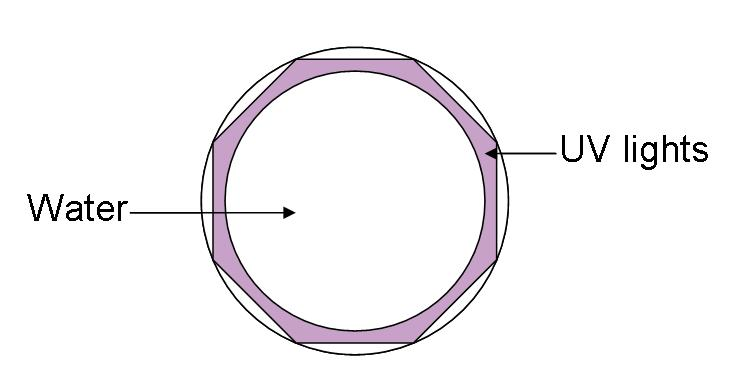
\includegraphics[width=4cm,height=2cm]{./images/coupeSterilisateur.jpg}
	\end{figure}
\item \textbf{Goal:} To find the optimal radius $r$ and $R$ for which :
	\begin{itemize} 
		\item[*] At the end of the pipe, the water is sterilized.
		\item[*] The flow must be 2 or 4 $l.min^{-1}$.
		\item[*] $R \in [7mm - 20mm]$ and $r \in [2mm - 6mm]$
	\end{itemize}
\item \textbf{Expected Result:} To create a computer program to search these radius.
\end{itemize}
\end{frame}



\subsection{Methodology}

\begin{frame}
	\frametitle{Methodology}
\begin{block}{Different concerned domains:}
\begin{itemize}[<+->]
\item Micro-Biology (bacteria's concentration)
\item Fluid Mechanics
\item Radiation
\end{itemize}
\end{block}
\pause
\invisible<1-2> {Our research approach: }
\begin{block}{Simplified case $\Rightarrow$ real case:}
\begin{itemize}[<+->]
\item 0D mean velocity
\item 1D mean velocity
\item 2D axisymmetric with a Poiseuille's Profile
\item 2D axisymmetric with simplified Navier-Stokes' equations
\end{itemize}
\end{block}
\end{frame}


\begin{frame}
	\frametitle{Methodology}
	\begin{figure}
		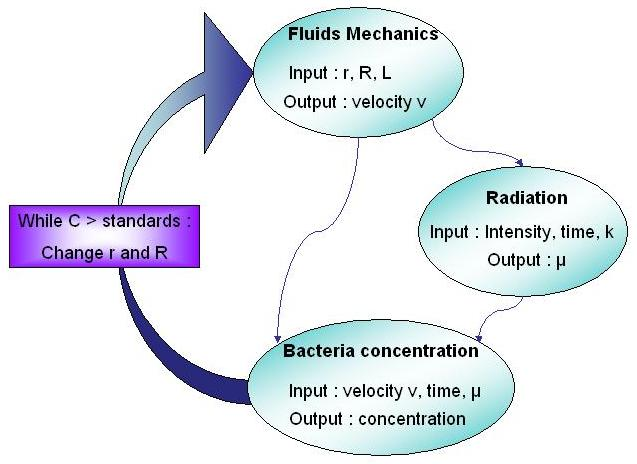
\includegraphics[width=9cm,height=7cm]{./images/methodology2.jpg}
	\end{figure}
\end{frame}

\subsection{Objectives}
\begin{frame}
\frametitle{Objectives}
\underline{\textbf{\color{blue}Frist:}}\\
\vspace{5mm}
$\Rightarrow$ To complete the 0D model before mid-Febrary.\\
\vspace{4mm}
$\Rightarrow$ To finish the 2D model and give representative results for $r$ and $R$ to obtain sterilized water.\\
\vspace{8mm}
\underline{\textbf{\color{blue}If miracle:}}\\
\vspace{5mm}
$\Rightarrow$ To do the same with the 3D model.\end{frame}


%%%%%%%%%%%%%%%%%%%%%%%%%%%%%%%%%%%%%%%% 0D %%%%%%%%%%%%%%%%%%%%%%%%%%%%%%%%%%%%%%%%%%%

\section{0 Space Dimension}

\subsection{Fluid Mechanics}

\begin{frame}
	\frametitle{The Darcy-Weisbach Equation}
		{\footnotesize
		\begin{itemize}
			\item RC-Lux gives us: the pressure loss $\Delta p$ 
			\item We look for: the velocity $v$ 
		\end{itemize}
		\begin{block}{The Darcy-Weisbach Equation (version 1)}
			\begin{equation}
				h_l = f \cdot \frac{L}{D} \cdot \frac{v^2}{2g}
			\end{equation}
		\end{block}
		where : 
	\begin{tabular}{ll}
		$h_l$: the head loss due to friction\\
		$f$: a Darcy friction factor\\
		$L$: the length of the pipe and $D$: the diameter of the pipe\\
		$g$: the gravitational constant
	\end{tabular}
		\begin{block}{The Darcy-Weisbach Equation (version 2)}
			Since $\Delta p = \rho g h_l$, where $\rho$ is the flow's density, we have :
			\begin{equation}
				\Delta p = f \cdot \frac{L}{D} \cdot \frac{\rho v^2}{2}
			\end{equation}
		\end{block}
}
\end{frame}

\begin{frame}
\frametitle{The Darcy Friction Factor}
	\begin{equation}
		\Delta p = \left(\sum_{p=1}^3 f_p\frac{L_p}{D_p} + K_e + K_c\right)\cdot \frac{\rho v^2}{2}
	\end{equation}
With : \\
\begin{block}{Swamee-Jain Equation}
\begin{equation}
	f_p = \frac{0.25}{[\log (\frac{\varepsilon}{3.7 D_p} + \frac{5.74\cdot \nu^{0.9}}{(v.D_p)^{0.9}})]^2}
\end{equation}
\end{block}
And : \\
\hspace{20mm}
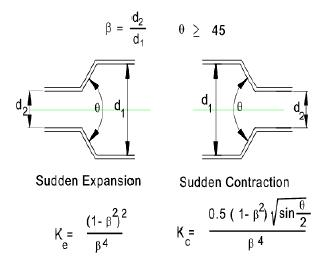
\includegraphics[height=25mm, width=5cm]{./images/fitting.JPG}
\end{frame}


\subsection{UV Radiation}

\begin{frame}
	\frametitle{UV Radiation}
\begin{block}{Single Stage Exponential Decay Equation}
	\begin{equation}
		S(t)=e^{-kIt}
	\end{equation}
\end{block}
Where 
	\begin{tabular}{ll}
		$S$: the surviving ratio of the initial population $\frac{c}{c_0}$\\
		$t$: the exposure time\\
		$I$: the UV radiation intensity\\
		$k$: the sensitivity coefficient of the microorganisms to UV exposure.
	\end{tabular}

\begin{figure}
	\raggedright
	
\includegraphics[height=0.5cm, width=0.6cm]{./images/warn.jpg}
\hspace{1mm} k is different for each bacteria species!
	\end{figure}
\vspace{2mm}
We choose to perform the simulation on a representative pathogen bacteria: the \textit{E. Coli}.
\end{frame}

\subsection{Bacteria's Concentration}

\begin{frame}
	\frametitle{Bacteria's Concentration}
In a first approximation:
 \begin{block}{Simplified Bacteria's Concentration Equation}
\begin{equation}
\left\{ \begin{array}{cl}
\frac{\partial{c}}{\partial{t}}= -\mu\cdot c\\
\\
c(t=0)=c_0
\end{array}
\right.
\end{equation}

 The solution of this problem is so: 
\begin{equation}
c(t) = c_0\cdot e^{-\mu t}
\end{equation}
\end{block}

Using the formula about radiation explained earlier, we obtain: 
\begin{block}{The Concentration at time t:}
\begin{equation}
c(t) = c_0\cdot S(t) = c_0\cdot e^{-kIt}
\end{equation}
\end{block}
\end{frame}


%%%%%%%%%%%%%%%%%%%%%%%%%%%% 2D %%%%%%%%%%%%%%%%%%%%%%%%%%%%%%%%%

\section{2 Space Dimensions}

\subsection{Fluid Mechanics}

\begin{frame}
	\frametitle{Fluid Mechanics}
		\begin{block}{Navier-Stokes Equations for incompressible flow}
			In axisymmetric coordinates with $\vec{u}$ the velocity and $p=p(r,z)$ the pressure.
			\begin{equation}
				\left\{ \begin{array}{cl}
				\frac{\partial \vec{u}}{\partial t} + \vec{u}\cdot \nabla \vec{u} - \nu\Delta\vec{u} + \nabla p = 0 \\
				\\
				div(\vec{u}) = 0
				\end{array}
				\right.
			\end{equation}
		\end{block}
\end{frame}

\subsection{UV Radiation}

\begin{frame}{UV Radiation}
We have : 
\begin{equation}
	S(t,r)=e^{-kI(r)t}
\end{equation}
With :
\begin{block}{The Beer-Lambert Law}
	\begin{equation}
		I(r) = I_0 \cdot e^{-\alpha r \rho}
	\end{equation}
\end{block}
\vspace{2mm}
	\begin{tabular}{ll}
		$I_0$: the intensity of the incident light\\
		$\alpha$: the absorption coefficient\\
		$r$: the distance to the light\\
		$\rho$: the water density.
	\end{tabular}
\end{frame}

\subsection{Bacteria's Concentration}

\begin{frame}
	\frametitle{Bacteria's Concentration}
\begin{block}{Bacteria's Concentration Equation}
\begin{equation}
\frac{\partial{c}}{\partial{t}} + \underbrace{\vec{u}\cdot \nabla c}_{advection} \underbrace{ - D(\vec{x},c)\cdot \Delta c}_{diffusion} + \underbrace{\mu\cdot c}_{reaction} = f
\end{equation}
\end{block}
Where,
\begin{tabular}{ll}
	$c$: the bacteria's concentration\\
	$u$: the fluid velocity\\
	$D(\vec{x},c)$: a coefficient given by simulation\\
	$\mu$: a constant which represents the bacteria's destruction
\end{tabular}
\end{frame}

%%%%%%%%%%%%%%%%%%%%%%%%%%%%%%%%%%%%%%%%%%%%Optimisation%%%%%%%%%%%%%%%%%%%%%%%%%%%%%%%%%%%%%%%%%%%%
\section{Optimization}

\subsection{Problem Formulation}
\begin{frame}
\frametitle{Problem Formulation}
\begin{block}{Formula}
\begin{equation}
\mathop{Min}\limits _{r\in [2,6];R\in [7,20];C<C_s} \alpha C(r,R) + \beta Vol(r,R) 
\end{equation}
\end{block}
\begin{itemize}
\item The dimension of the radius is the millimeter.\\
\item We use $\Delta p = kQ^2$ to have the constraint on the flow.
\end{itemize}
\end{frame}

\subsection{First Approximation}
\begin{frame}
\frametitle{First Approximation : $\beta = 0$ and $r=2mm$ $\Rightarrow \mathop{Min}\limits _{R\in [7,20]} C(R)$}
\begin{block}{Formula}
\begin{equation}
\left(f_1(v)\frac{L_1+L_3}{2r} + f_2(v,R)\frac{L_2}{2R} + K_e + K_c\right)\cdot \frac{\rho v^2}{2} - \Delta p = 0
\end{equation}
\begin{equation}
c(R) = c_0\cdot e^{-kI\frac{L_2}{v(R)}}
\end{equation}
\end{block}
$1^{st}$ Step : $v(R)$ \hspace{30mm} $2^{nd}$ Step : $C(R)$
	\begin{figure}
	\raggedleft
	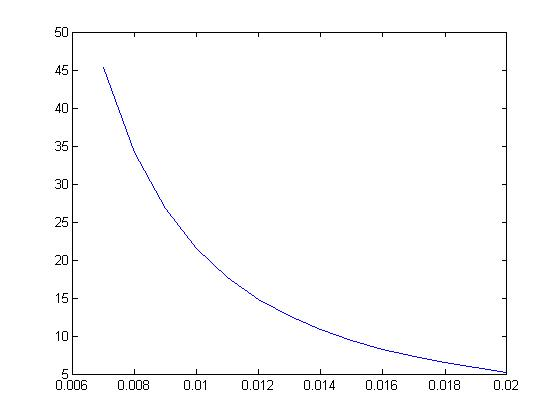
\includegraphics[height=3.1cm, width=5cm]{./images/graphVR.jpg}
	\hspace{5mm}
	\raggedright
	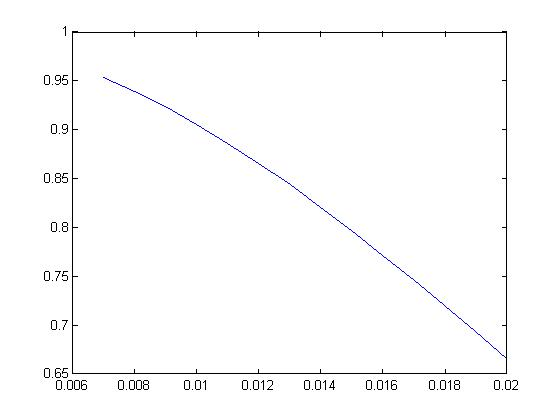
\includegraphics[height=3.1cm, width=5cm]{./images/graphCR.jpg}
	\end{figure}
\end{frame}

\subsection{In the Future}
\begin{frame}
\frametitle{In the Future}
\begin{itemize}
\item 0 Space Dimension :
	\begin{itemize} 
		\item[*] To find the minimum bacteria concentration with $r$ and $R$.
		\item[*] To optimize with the volume
	\end{itemize}
\vspace{1cm}
\item 1 Space Dimension
\vspace{1cm}
\item 2 Space Dimension

\end{itemize}
\end{frame}

%%%%%%%%%%%%%%%%%%%%%%%%%%%%%Conclusion%%%%%%%%%%%%%%%%%%%%%%%%%%%%%%%%%%%%

\section{Conclusion}

\begin{frame}
	\frametitle{Conclusion}
\underline{\textbf{\color{blue}Negative Points:}}\\
 \begin{itemize}
  \item Delay in our schedule.
  \item More complex than we expected.
  \item Almost no communication with the RC-Lux company.
  \end{itemize}

\underline{\textbf{\color{blue}Positive Points:}}\\ 
 \begin{itemize}
  \item Very interesting and concrete subject with different scientific domains.
  \item Learning of many things.
  \item Participation to an industrial project.
 \end{itemize}
\end{frame}

\begin{frame}
\vspace{8mm}
\hspace{4mm}
\huge{\textbf{\color{blue}Thank you for your attention}}
\end{frame}

\end{document}

%\begin{frame}
%	\frametitle{3 Space Dimensions Model}
%		\begin{block}{Navier-Stokes Equations for incompressible flow}
%			In Cartesian coordinates with $(u,v,w)$ the velocity and $p=p(x,y,z)$ the pressure.
%			\begin{equation}
%				\left\{ \begin{array}{cl}
%				\frac{\partial u}{\partial t} + u\frac{\partial u}{\partial x} + v\frac{\partial u}{\partial y} + w\frac{\partial u}{\partial z} = -\frac{1}{\rho}\frac{\partial p}{\partial x} + \nu(\frac{\partial^2 u}{\partial x^2}+\frac{\partial^2 u}{\partial y^2}+\frac{\partial^2 u}{\partial z^2})+g_x \\
%				\\
%				\frac{\partial v}{\partial t} + u\frac{\partial v}{\partial x} + v\frac{\partial v}{\partial y} + w\frac{\partial v}{\partial z} = -\frac{1}{\rho}\frac{\partial p}{\partial y} + \nu(\frac{\partial^2 v}{\partial x^2}+\frac{\partial^2 v}{\partial y^2}+\frac{\partial^2 v}{\partial z^2})+g_y \\
%				\\
%				\frac{\partial w}{\partial t} + u\frac{\partial w}{\partial x} + v\frac{\partial w}{\partial y} + w\frac{\partial w}{\partial z} = -\frac{1}{\rho}\frac{\partial p}{\partial z} + \nu(\frac{\partial^2 w}{\partial x^2}+\frac{\partial^2 w}{\partial y^2}+\frac{\partial^2 w}{\partial z^2})+g_z \\
%				\\
%				\frac{\partial u}{\partial x} + \frac{\partial v}{\partial y} + \frac{\partial w}{\partial z} = 0
%				\end{array}
%				\right.
%			\end{equation}
%		\end{block}
%\end{frame}

%\section{Numerical Methods and programming language choice}

%\subsection{Numerical methods}

%\begin{frame}
%	\frametitle{Optimization}
%  \begin{itemize}
%  \item<1-> Problem can be expressed as
%		\begin{equation}
%		\mathop{\rm Min}\limits _{(r,R,L,P_{in})} f(r,R,L,P_{in})
%		\end{equation}
%		$f$ : Functional to minimise
%  \item<2-> Maximise time required to cross the pipe $f \equiv time$
%		\begin{tabular}{ll}
%		$f  =$ & $ \frac{L}{U}$\\
%		$U$ : & Celerity of the fluid 
%		\end{tabular}
%  \item<3-> Minimise bacteria concentration
%		$$\frac{\partial c}{\partial t} -\nu \Delta c  + \vec{u} \cdot \nabla c + \mu c = g$$
%		\begin{tabular}{ll}
%		$c$ : & Bacteria concentration\\
%		$U$ : & Celerity of the fluid \\
%		$g$ : & Source term which we'll suppose null $(g \equiv 0)$
%		\end{tabular}
%  \end{itemize}
%\end{frame}

%\begin{frame}
% \frametitle{Algebraic Equation}
%  \begin{itemize}
%  \item<1-> Bernoulli's equation
%		\begin{equation}
%		{U^2 \over 2g}+h+{p \over \rho g}= H
%		\end{equation}
%		$H$ : Hydraulic head  
%	\item<2-> Head loss due to friction
%		\begin{equation}
%		H_l = f \cdot \frac{L}{D} \cdot \frac{U^2}{2g}
%		\end{equation}
%	\item<3-> Head loss and pressure drop
%		\begin{equation}
%		 \Delta p = \rho g H_l
%		\end{equation}
%  \end{itemize}
%\end{frame}

%\begin{frame}
%  \frametitle{Algebraic Equation (Sequel)}
%  \begin{itemize}
%  \item Darcy-Weisbach equation for pipes 
%		\begin{equation}
%		h_f = \left(\sum_{p=1}^P K_p + \sum_{l=1}^{P-1} K_l\right) \frac{U^2}{2 g}
%		\end{equation}

%		$K_p = f_p \frac{L_p}{D_p}$\\
%\raggedleft
%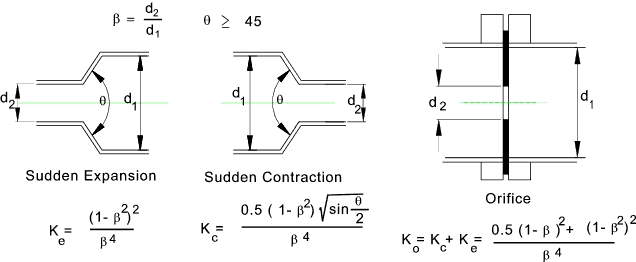
\includegraphics[height=4cm, width=8cm]{./images/fittings.JPG}

%  \end{itemize}
%\end{frame}

%\begin{frame}
%\frametitle{Algebraic Equation (Sequel)}
%  \begin{itemize}
%  \item<1-> Colebrook-White equation
%		\begin{equation}
%		\frac{1}{\sqrt{f}} = -2 \log (\frac{\varepsilon}{3.71 D} + \frac{2.51}{Re\sqrt{f}})
%		\end{equation}
%  \item<2-> Swamee-Jain equation
%		\begin{equation}
%		f = \frac{0.25}{[\log (\frac{\varepsilon}{3.7 D} + \frac{5.74}{Re^{0.9}})]^2}
%		\end{equation}
%	\item<3-> Velocity computation
%		\begin{equation}
%		\left(\sum_{p=1}^P f_p(U) \frac{L_p}{D_p} + \sum_{l=1}^{P-1} K_l\right) \frac{U^2}{2}-\Delta p = 0
%		\end{equation}
%  \end{itemize}
%\end{frame}

%\subsection{Programming Language Choice}

%\begin{frame}
%  \frametitle{Programming Language choice}

%  \begin{itemize}
%  \item<1-> lifev
%  \item<2-> FreeFem++, FreeFem3D
%  \end{itemize}
%\end{frame}

%\begin{frame}
%	\frametitle{Conclusion}
%What we have done : 
% \begin{itemize}
%  \item Litterature review
%  \item Modeling and optimisation in 0 dimension in space and 1 in time
%  \item Found all types of equations we need for radiation and concentration
%  \end{itemize}
 
%What we have to do : 

% \begin{itemize}
%  \item Meet RC-Lux engineers and specialists to validate or not our choices
%  \item Modeling in 2 dimensions in space water passing, radiation and bacteria's concentration
%  \item Implement code for optimisation in 2D case
%  \item Same for 3D case 
%  \end{itemize}
%\end{frame}
